\newpage 
\appendix
\section{Appendix}

\subsection{Example of current chatbots' ability to combine skills}
\label{appendix:gpt_examples}
We find that current chatbots, including those in the public domain, can take a list of language skills and produce text illustrating those skills. When the list includes harder (or less common) skills, this ability  declines. We include an illustrative example but a more thorough evaluation is left to future work.



\iffalse
\begin{tabular}{|p{6cm}|p{10cm}|}
\hline
\textbf{Language Understanding Skills} & \textbf{Illustrative Text} \\
\hline
Anaphora resolution, simple logical reasoning, simple understanding of physics, and understanding of sentiment & As the car skidded on the icy road, the driver desperately gripped the wheel, trying to regain control. In that tense moment, their heart raced, fearing the imminent collision and praying for a safe escape. \\
\hline
\end{tabular}
\fi

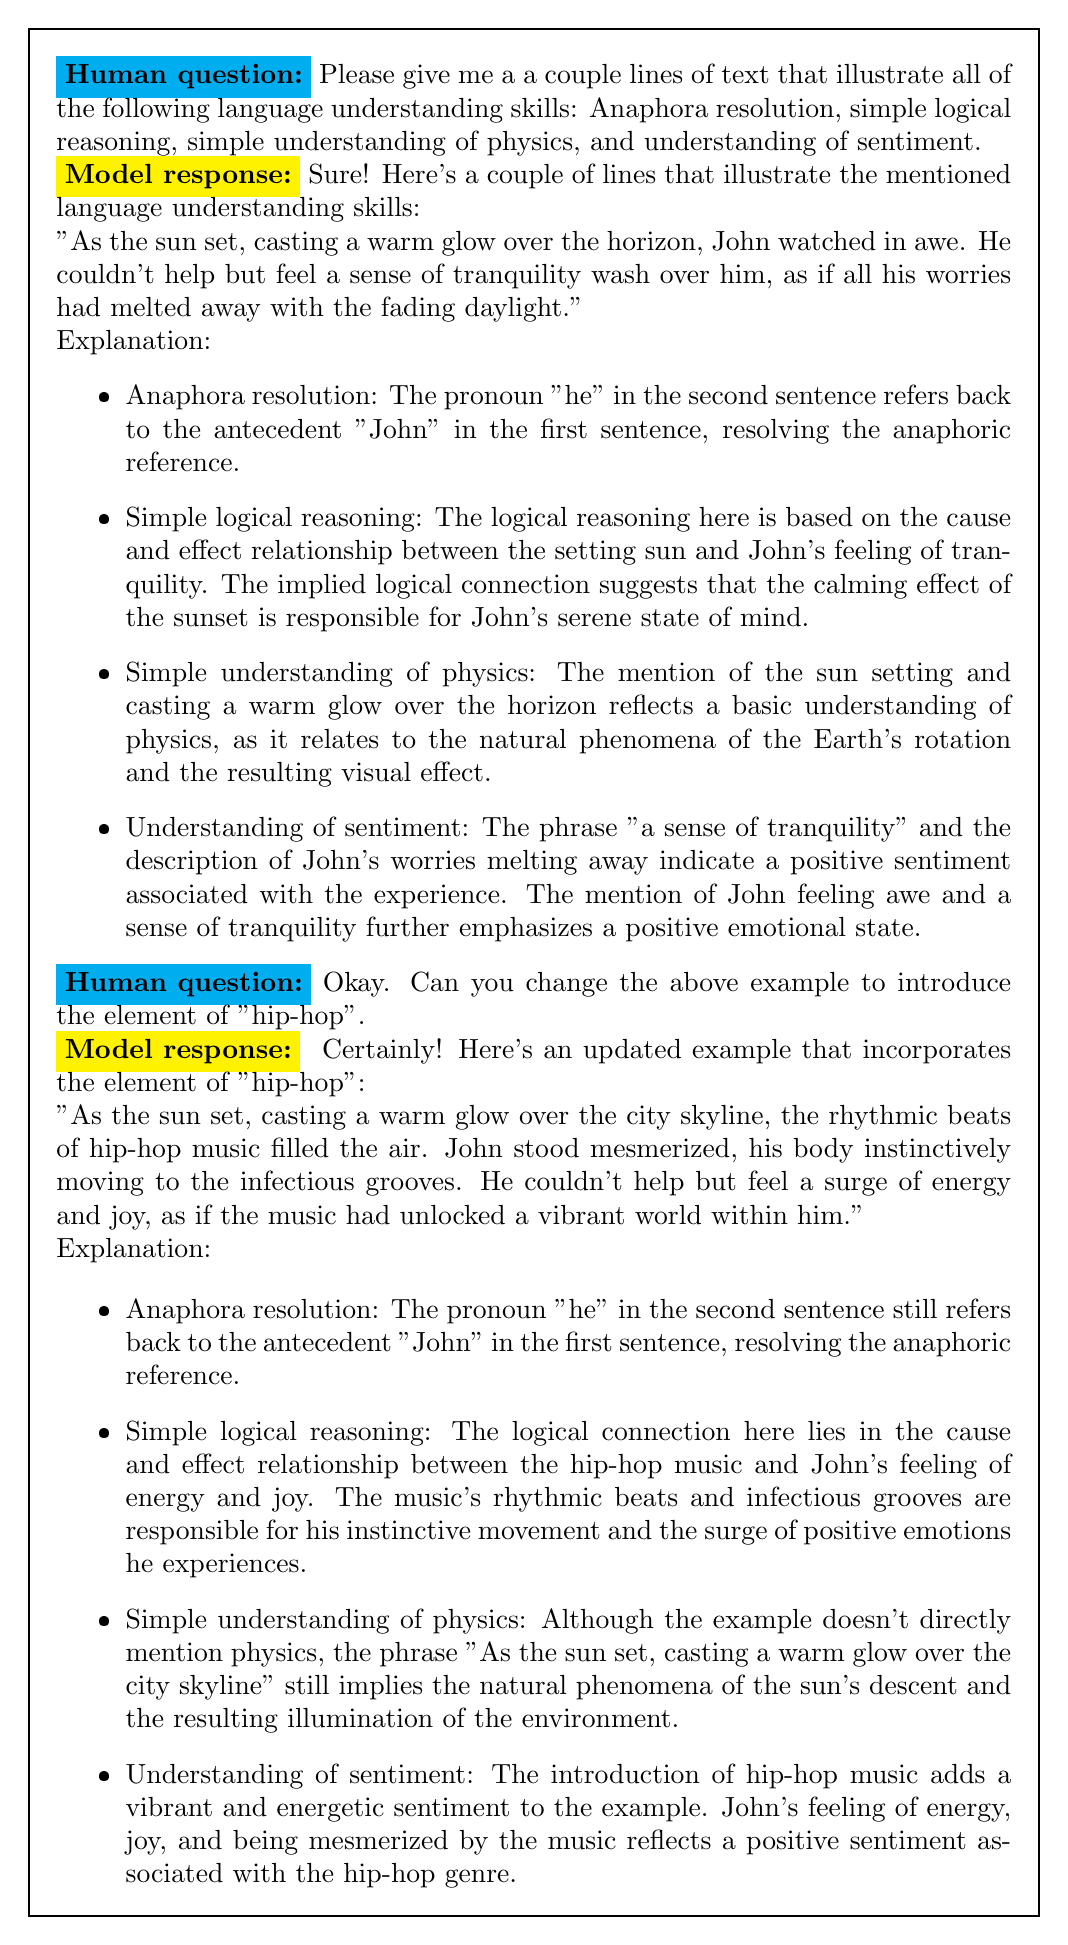
\begin{tikzpicture}
\node[rectangle, draw=black, thick, inner sep=10pt]{
\begin{minipage}{\textwidth}

\colorbox{cyan}{\textbf{Human question:}}  Please give me a a couple lines of text that illustrate all of the following language understanding skills: Anaphora resolution, simple logical reasoning, simple understanding of physics, and understanding of sentiment.

\colorbox{yellow}{\textbf{Model response:}}  Sure! Here's a couple of lines that illustrate the mentioned language understanding skills:

"As the sun set, casting a warm glow over the horizon, John watched in awe. He couldn't help but feel a sense of tranquility wash over him, as if all his worries had melted away with the fading daylight."

Explanation:
\begin{itemize}
    \item Anaphora resolution: The pronoun "he" in the second sentence refers back to the antecedent "John" in the first sentence, resolving the anaphoric reference.
    \item Simple logical reasoning: The logical reasoning here is based on the cause and effect relationship between the setting sun and John's feeling of tranquility. The implied logical connection suggests that the calming effect of the sunset is responsible for John's serene state of mind.
    \item Simple understanding of physics: The mention of the sun setting and casting a warm glow over the horizon reflects a basic understanding of physics, as it relates to the natural phenomena of the Earth's rotation and the resulting visual effect.
    \item Understanding of sentiment: The phrase "a sense of tranquility" and the description of John's worries melting away indicate a positive sentiment associated with the experience. The mention of John feeling awe and a sense of tranquility further emphasizes a positive emotional state.
\end{itemize}

\colorbox{cyan}{\textbf{Human question:}}  Okay. Can you change the above example to introduce the element of "hip-hop".

\textbf{\colorbox{yellow}{\textbf{Model response:}} } Certainly! Here's an updated example that incorporates the element of "hip-hop":

"As the sun set, casting a warm glow over the city skyline, the rhythmic beats of hip-hop music filled the air. John stood mesmerized, his body instinctively moving to the infectious grooves. He couldn't help but feel a surge of energy and joy, as if the music had unlocked a vibrant world within him."

Explanation:

\begin{itemize}
\item Anaphora resolution: The pronoun "he" in the second sentence still refers back to the antecedent "John" in the first sentence, resolving the anaphoric reference.
\item Simple logical reasoning: The logical connection here lies in the cause and effect relationship between the hip-hop music and John's feeling of energy and joy. The music's rhythmic beats and infectious grooves are responsible for his instinctive movement and the surge of positive emotions he experiences.
\item Simple understanding of physics: Although the example doesn't directly mention physics, the phrase "As the sun set, casting a warm glow over the city skyline" still implies the natural phenomena of the sun's descent and the resulting illumination of the environment.
\item Understanding of sentiment: The introduction of hip-hop music adds a vibrant and energetic sentiment to the example. John's feeling of energy, joy, and being mesmerized by the music reflects a positive sentiment associated with the hip-hop genre.
\end{itemize}

\end{minipage}
};
\end{tikzpicture}


\section{Technical Theorems about Random Bipartite Graphs}

\label{sec:randomgraphs}
The theory will need some facts about random bipartite graph $(V_1, V_2, E)$  with $N_i$ denoting $|V_i|$, and $N_1 \gg N_2$. 
When we say it has degree $k$, we mean that in $E$ every vertex in $N_1$ is connected to $k$ vertices in $N_2$, where those $k$ vertices are chosen i.i.d.\ with replacement. Recall that $V_1$ corresponded to text-pieces and $V_2$ to skills in the main body of the paper.
In the next Lemma, the important thing to note is that a property is established for {\em all} subsets of a certain size, not just many/most subsets.  

\begin{lemma}[Main]\label{lem:mixing}
    For every positive integer $k$ and $\theta \in [0,1]$  there are $\alpha, \beta >0$ such that $\alpha \beta \leq 1$ and the following holds with probability almost $1$. For every $Y \subseteq V_1$ of size $\theta N_1$, there are at least   $(1-\alpha)$ fraction of vertices in $V_2$ each of which has  at most $\beta \theta D$ edges going to $Y$, where $D =kN_1/N_2$. The parameter values for which this occurs are specified by the condition
\begin{equation} \label{eqn:mix2b}
    H(\theta) + k\theta (H(\beta \alpha)  - \beta \alpha  \log \frac{1}{\alpha} - (1- \beta \alpha)  \log (\frac{1}{1-\alpha}))<0
\end{equation}\end{lemma}
\begin{proof}
As is standard in random graph theory and the Probabilistic Method~(\cite{alonspencer}) it suffices to show that the the expected number of subsets of size  $\alpha N_2$ satisfying the opposite property is $o(1)$: In other words, the number of $Z \subseteq V_2$ of size $\alpha N_2$  and have at least $\alpha \beta \theta k N_1$ edges to $Y$.  The expected number of these $Z$'s is upper bounded by 
\begin{equation} {N_2 \choose \alpha N_2} \times {N_1 \choose \theta N_1} \times {k\theta N_1 \choose \beta \alpha k \theta  N_1} \times \alpha^{\beta \alpha \theta k N_1} \times (1-\alpha)^{(1-\beta \alpha )\theta kN_1} \label{eqn:mix1} \end{equation}
For (\ref{eqn:mix1}) to be $\ll 1$ it suffices for its logarithm to be negative. In such such calculations in random graph theory it is standard (and rigorous) to use the approximation ${N \choose t N} = 2^{H(t)N}$ where $H(t)= - t\log t - (1-t)\log (1-t) $ is the entropy function. Applying this to (\ref{eqn:mix1}) and  taking logarithms, and assuming $N_2 \ll N_1$, we  arrive at the condition (\ref{eqn:mix2}). 
%The plots in Appendix Section~\ref{??} show that the above inequality has a continuous set of solutions. As $k$ gets larger, $\beta \rightarrow 1$ even for small $\alpha$. Figure~\ref{fig:mixing_lemma} gives the plot for $\theta =0.7, k=3$ (the best $\alpha, \beta$ combinations lie along the countour between red and blue).
\end{proof}

\subsection{Analysis of ``General Measure'' case in Section~\ref{subsec:measure}}

We give more details of the proof of Theorem~\ref{thm:genmeasure} in Section~\ref{subsec:measure}.
Again, we phrase it via a general lemma about bipartite graph 
$(V_1, V_2, E)$ where each vertex in $V_1$ has edges to $k$ random vertices in $V_2$. We use the shorthand $N_i =|V_i|$. As noted in proof of Theorem~\ref{thm:genmeasure} it suffices to consider the case when $V_2$ has uniform measure and there is a general measure $\mu()$  on vertices of $V_1$. By our assumptions about marginals of $\mu()$ this means 
%\footnote{The way to think of this is that text is generated by taking a random $k$-tuple of skills and using it to generate a piece of text. Then nature attaches a probability to the piece of text.} 
 $\mu(v_1)$ is nonnegative and $\sum_{v_1 \in V_1} \mu(v_1) =1$. The measure of an edge $(v_1, v_2)$ is defined as $\mu(v_1)$. We assume all  $\mu(v_1)$ are sufficiently small.

The proof will use a discretization of the measure. We conceptually divide $V_1$ into {\em classes}, where the $i$th class  consists of 
$v_1$ such that $\mu(v_1) \in [(1+\epsilon)^{-i -1}, (1+\epsilon)^{-i})$ for $\epsilon$ an arbitrarily small constant. We assume all  $\mu(v_1)$ are sufficiently small (meaning some large-ish $i_0$, class $i$ is empty for $i < i_0$) and the number of nonempty levels is much smaller than $N_1$. Thus each class has reasonable size ---say,  much larger than $N_2$---which allows  the asymptotic arguments appearing below to hold within each class.  
 The above assumptions all seem reasonable for the probability measure associated with text pieces, which should be fairly well spread out.

\begin{lemma}[Main]\label{lem:mixing+measure}
     For every positive integer $k$ and $\theta \in [0,1]$  and $\alpha, \beta >0$ satisfying $\alpha \beta \leq 1$ and 
    \begin{equation} \label{eqn:mix2}
    H(\theta) + k\theta (H(\beta \alpha)  - \beta \alpha  \log \frac{1}{\alpha} - (1- \beta \alpha)  \log (\frac{1}{1-\alpha}))<0
    \end{equation}
    the following holds with probability almost $1$ in the random bipartite graph $(V_1, V_2, E)$ of degree $k$:

 For every $Y \subseteq V_1$ of total measure $\theta$, there is a set of least   $(1-\alpha)$ fraction of vertices in $V_2$ such that  for each $v_2$ in this set, % the measure of edges incided to $v_2$ that lie in $$
\begin{equation}
    \sum_{v_1: (v_1,v_2) \in E, v_2 \in Y}\mu(v_1) \leq \beta \theta. \label{eqn:failm1}
\end{equation} \end{lemma}
\begin{proof}
  Consider $Y  \subseteq V_1$ that has measure $\theta$, and $Z \subseteq V_2$ has size $\alpha N$. We say   $(Y, Z)$  is {\em bad} if every $v_2 \in Z$ fails condition (\ref{eqn:failm1}). (Consequently, the measure of edges between $Z$ and $Y$ is at least $\alpha \beta \theta$.) We will argue that in the random graph, the expected number of bad $(Y, Z)$ is $\ll 1$. In other words, for any fixed measure $\mu$ with high probability the graph contains no bad $(Y, Z)$.

 

For any fixed $Y \subseteq V_1$ we denote by $Y_i$ its intersection with the $i$th class and also let $y_i =|Y_i|$.
Since $\mu(Y) =\theta$ the $y_i$'s satisfy 
\begin{equation}
    \sum_i y_i (1+\epsilon)^{-i} \approx \theta \qquad \label{eqn:failm2}
\end{equation} 


For a fixed $(Y, Z)$ let $\beta_i$ be such that the number of edges between $Y_i, Z$ is $\alpha \beta_i y_ik$. Then the probability (over the choice of the random graph) that $(Y, Z)$ is bad is at most:
\begin{equation}
    \label{eqn:mixm3}
    \prod_i {ky_i \choose \alpha \beta_i ky_i}(\alpha)^{-\alpha \beta_i y_i}(1-\alpha)^{ky_i(1 -\alpha\beta_i)} 
\end{equation}
Since $\sum_i y_i =|Y|$ and ${ky_i \choose \alpha \beta_i ky_i} \approx 2^{H(\alpha \beta)ky_i}$, this expression is maximized when all $\beta_i$ are equal. (NB: This used the concavity of the entropy function.) So for deriving an upperbound it suffices to let all $\beta_i =\beta$,
which simplifies the expression to
\begin{equation}
    \label{eqn:mixm4}
    \prod_i {ky_i \choose \alpha \beta ky_i}(\alpha)^{-\alpha \beta y_i}(1-\alpha)^{ky_i(1 -\alpha\beta)} \approx 2^{H(\alpha \beta)k|Y|} (\alpha)^{-\alpha \beta |Y|}(1-\alpha)^{k|Y|(1 -\alpha\beta)} .
\end{equation}
%where we have used the usual approximation of ${n \choose t n} \approx 2^{H(t)n}$. 
Now we finish the proof using reasoning similar to that in Lemma~\ref{lem:mixing}. We show that when we pick a random $(Y, Z)$ then the expected number of bad $(Y, Z)$ pairs is $\ll 1$. %Let the classes for measure $\mu$ be defined as above, and suppose $C_i$ is the set of $v_i$'s in $i$th class. 
We pick a random $Y$ as follows: pick each $v_1 \in V_1$ with probability $\theta$. Under our assumption about no $v_1$ having very large $\mu(v_1)$ this way of picking gives roughly equal probability to all subsets with measure $\theta$ and $\exp(-\Omega(N_1))$ to subsets of measure fairly different from $\theta$. So up to a small multiplicative error of $\exp(-\epsilon N_1)$ (which after taking logarithm affects (\ref{eqn:mix2}) by an additive term $\epsilon$) we are taking expectation over exactly the subsets of measure almost exactly $\theta$. 

If $C_i$ is the number of $v_1$'s in the $i$th class, then with high probability $|Y_i| \approx \theta |C_i|$ for all $i$. Thus the number of sets of measure $\theta$ is approximately $\prod_i {|C_i| \choose \theta |C_i|} = 2^{H(\theta)N_1}$.
By the union bound, the probability that there exists a $Y$ such that  $(Y, Z)$ is bad is at most $2^{H(\theta) N_1}$ times (\ref{eqn:mixm4}), and since $|Y| \approx \theta N_1$ this completes the proof of Lemma~\ref{lem:mixing+measure}.
\end{proof}

 % Let ${\mathcal Y}$ be the set of  $ Y \subseteq V_1$ with $\mu(Y) \leq \theta$.  To let the calculation in (\ref{lem:mixing}) go through it suffices to show that the number of such subsets is at most $2^{(1+o(1))H(\theta) N_1}$, where $o(1)$ is a term that goes to $0$ as $N_1 \rightarrow \infty$.
  
  %Lacking a clean way of sampling a random $Y$ uniformly from ${\mathcal Y}$ we describe  a more general probability distribution ${\mathcal D}$  over subsets of $V_1$ such that $\Omega(1/N)$ fraction of the probability in this distribution is over $Y$ with  $ \mu(Y) =\theta$. This is simple the distribution where each $v_1 \in V_1$ is included independently with probability $\theta \mu(v_1) N_1$, and which defines a distribution over subsets of $V_1$ where the probability assigned to $Y \subseteq V_1$, is 
%$\prod_{v_1 \in Y}(\mu(v_1) \theta N_1) \prod_{v_1 \not \in Y}(1-\mu(v_1) \theta N_1).$    
%\end{proof}
\iffalse
% Figure environment removed
\fi
